\documentclass[11pt]{article}

\usepackage[]{graphics}
\usepackage{natbib}
\usepackage[margin=2cm]{geometry}
\usepackage{hyperref}
\usepackage{url}
\usepackage{enumitem}
\usepackage{titlesec}
\usepackage{pgfgantt}


\setlist[enumerate]{itemsep=0mm, parsep=0mm}
\setlist[itemize]{itemsep=0mm, parsep=0mm}

\titleclass{\subsubsubsection}{straight}[\subsection]

\newcounter{subsubsubsection}[subsubsection]
\renewcommand\thesubsubsubsection{\thesubsubsection.\arabic{subsubsubsection}}
\titleformat{\subsubsubsection}
  {\normalfont\normalsize\itshape}{\thesubsubsubsection}{1em}{}
\titlespacing*{\subsubsubsection}
{0pt}{3.25ex plus 1ex minus .2ex}{1.5ex plus .2ex}

\makeatletter
\def\toclevel@subsubsubsection{4}
\def\l@subsubsubsection{\@dottedtocline{4}{7em}{4em}}
\makeatother

\setcounter{secnumdepth}{4}
\setcounter{tocdepth}{4}



%opening
\title{Developing an Intelligent Chatbot}
\author{Group 18: Alexander Vranic* - 100350592, James Hamilton - 100340006}




\begin{document}

\maketitle


\begin{abstract} \label{abstract}
% This interim report presents (1) the outline of our coursework report, (2) some initial descriptions of the requirements of the coursework, the methods, programming languages, packages, tools that have been identified so far, and (3) an initial work plan.
    ABSTARACTIONS

\end{abstract}




\section{Introduction} \label{introduction}

In recent years, chatbots have become increasingly popular in a variety of applications, as such, so has the technology surrounding them. It is not our mission to compete with the likes of \cite{openai}, \cite{microsoft} and \cite{github} and their hugely successful Large Language Models (LLMS), GPT-4 \cite{gpt4} and CoPilot \cite{copilot} respectively. At the end of the day, the coursework is a learning experience, not a fully fledged product.

Our solution is a small client side chatbot, integrated into an intuitive graphical user interface and designed to handle prompts around a bespoke context. We utilise modern natural language processing (NLP) techniques, with a knowledge base and inference engine, with machine learning and webscraping, in the name of enabling the user with concurrent information to make informed decisions on their train travel plans.


\subsection{Background and Motivation} \label{background}

\subsubsection{Compulsory Motivators (Assignment Brief)} \label{compulsory-motivators}

As specified in the CMP6040/7028 assignment brief \cite{AI2018CW}, tasks one and two are to implement an intelligent conversational system, designed to "\textit{help their customers in finding the cheapest available ticket for their chosen journey}" covered by section \ref{task1-aims-objectives} and "\textit{to improve customer service satisfaction by applying some appropriate AI techniques}" covered by section \ref{task2-aims-objectives} respectively. Following implicit suggestions from the course contents, our second task implements a delay prediction model, based on historical data (also provided in the course material), in the form of a KNN regressor (\cite{knn-origin}), embedded within the original chatbot system created in task one. In depth coverage of our interpretation of the brief seen in section \ref{task1-aims-objectives}.

Again, as stated in the brief, we are to provide some kind of user interface. Seeing that with our resources, any web based applications would be limited to local hosting anyway, we have decided to create a stand alone desktop application with a graphical user interface (GUI) to mimic the look and feel of modern chat applications. For further clarification, see section \ref{task2-aims-objectives}.

\subsubsection{Chatbot History} \label{chatbot-history}

Quite some time before the advanced development of AI chatbots, Alan Turing considered the idea of a hypothetical machines ability to think, proposing a method of benchmarking a machines intelligence, aptly named "\textit{The Imitation Game}" \cite{turing1950}, not to be confused with the Turing Test - being the broader concept of measuring a systems intelligence. In the paper, Turing proposed a system involving three parties: a human interrogator, a human respondent and a machine respondent. The core concept being that the human interrogator must converse with both responding parties and determine which is the machine. The machine is deemed intelligent if it is not reliably distinguished from the human respondent. Turing states that "\textit{at the end of the century}" - being the year 2000 - "\textit{one will be able to speak of machines thinking without expecting to be contradicted}". Though the timing of his prediction can be argued either way, the concept of a machine being able to hold conversation with a human is now a reality, to the point where as a modern humans, we must be consciously question the \textit{human-made} authenticity of the content and media we consume.

Artificial intelligence, designed to mimic human conversation has come a long way since the days of Turing. From the first chatbot ELIZA \cite{eliza} providing incoherent responses diverged from context, to today's CoPilot \cite{copilot} baring the capability to generate code and explain it in any array of natural languages, the technology has become an integral part of our daily lives.


\subsection{Aim and Objective} \label{aim-objective}

As I'm sure you're aware by this point in the report, we are to employ artificial intelligence techniques, in conjunction with webscraping to achieve the following two tasks (\cite{AI2018CW}), with data relevant to the current and/or user-specified time frame(s).

\begin{enumerate}
    \item Finding the cheapest train ticket
    \item Improving Customer Service
\end{enumerate}

The following subsections \ref{task1-aims-objectives} and \ref{task2-aims-objectives} outline our subjective interpretation of the task one and two respectively. 

\subsubsection{Task 1: Finding the Cheapest Ticket} \label{task1-aims-objectives}

We've taken it upon ourselves to not just find the cheapest individual ticket, but to find the cheapest combination of tickets for a given journey. Once information is derived and tokenised, we achieve this by scraping the SplitMyFare website \cite{splitmyfare}.

Seeing that their service does incur a small additional fee, initial intentions were to then compare the results from another source, such as Trainline \cite{trainline}, to ensure the cheapest pricing of single ticket journeys. However, it would seem that these websites are intentionally or unintentionally difficult to scrape information from, as such, focus was shifted to the components relevant to the names sake of the module. Evidence for which is covered in sections \ref{work-plan} and \ref{design}, as well as the actual codebase itself\\ \textit{./webscrape/nationalrail.py} \cite{repo}.

As for how this determines the functionality of the actual chatbot. Our system should prompt the user with a series of reactive questions to derive the following information.

\subsubsubsection{Information To Derive}
\begin{itemize}
    \item Desired starting location
    \item Desired destination location
    \item Whether to arrive or depart by a certain time
    \item User specified time and date of departure or arrival
    \item Number and type of passengers (adults or children)
    \item Whether they want a return journey
        \begin{itemize} \item If so, then repeat the above, minus passengers \end{itemize}
\end{itemize}

Said information is to be, processed by a natural language processing algorithm, covered in section \ref{nlp-design}, with the resulting tokens updating the state machine responsible for determining its next prompts, until it reaches a completion state. Conversational control covered in section \ref{dialogue-flow-design}.

On arrival of a completion state, these tokens are to be formatted into a consistent data format, to be passed to the webscraping module, covered in section \ref{webscraping}. The results are then returned to the user via the GUI, covered in section \ref{user-interface-design}.

\subsubsection{Task 2: Improving Customer Service} \label{task2-aims-objectives}

Given historical performance data from years 2017 to 2022 for the service from London Liverpool Street to Norwich, we aim to provide a prediction for a \textit{actual} delayed time of arrival for journeys either direction between Norwich and London Liverpool Street, given the journey's current locational and time data for comparison to that of the historical data. With a machine learning algorithm known as K Nearest Neighbours (KNN), first publish in paper \cite{knn-origin} and later refined in \cite{knn-refine}.

KNN being a simple yet effective algorithm for regression and classification problems, with applications in pattern recognition, we thought it sufficient for the task at hand. It's to be noted that it is a lazy learning algorithm, so works by memorisation of the training data, rather than learning a discriminative function. Regardless, see our coverage of its implementation in section \ref{dialogue-flow-design}.

The chatbot aspect is to prompt and process user input in much the same way as task one, with different tokenisation parameters and completion states. Again coverage seen in sections \ref{dialogue-flow-design}.

\subsubsubsection{Information To Derive}
\begin{itemize}
    \item Current time and date
    \item Current journey direction
    \item Current/last know station location
    \item Current predicted delay time given by service provider
\end{itemize}

This time the appropriate tokens are to be processing into a consistent data format to be passed to the KNN regressor, from which the results can be displayed to the user through user interface, covered in section \ref{user-interface-design}.


\subsection{Difficulties and Risks} \label{difficulties-risks}

As is the case on any scale of software development, there are always factors that bare the potential to hinder progress. The following sections ....... outline the obstacles we aim to take particular to navigate.

\subsubsection{Mismatching Operating Systems} \label{mismatching-os}

With one member using Windows 11 \cite{windows}, and the other using Fedora Linux \cite{fedora}, there is potential for one of us to write or import code that the other cannot execute. Our simple solution is to use only cross platform tools and libraries for development, execution and testing of our codebase. Our choices of which are covered in sections \ref{languages-packages-tools}.

\subsubsection{Unacceptable Range of Output} \label{unacceptable-output}

\subsubsubsection{NLP Tokenisation and Responses} 
In developing our solution to task one, we'll be bound to come across issues regarding defining our ruleset's for the NLP state machine. This is to be considered regarding our time management, though through careful planning and testing, the time deficit can be minimised.

\subsubsubsection{KNN Regressor}
Without actually implementing the solution, we are yet to see if the model passes our specifications outlined in section \ref{delay-prediction-design}. If the model is not accurate enough, we may have to consider a more complex model, which could take more time to implement, train and test. All things to consider in our time management covered in section \ref{work-plan}.

\subsubsection{Webscraping Deterance Technologies} \label{webscrape-deterance}
It's no secret that scraping this information from SplitMyFare's online services is not something they wish to facilitate. Ultimately, between dynamic content (with arbitrary class names and tag ids, generated by frameworks like React \cite{react}) and other security measures in place to specifically prevent scraping, time is to be allocated to the development of a robust webscraping module, covered in section \ref{webscraping-design}.


\subsection{Work Plan} \label{work-plan}

\begin{ganttchart}[
        vgrid={*{5}{gray, dotted}, *1{black, dashed}},
        bar label node/.append style={align=left, text width=width("Aim 2. Software verificationx")},
        x unit=1.36cm,
        y unit chart=0.6cm,
        bar height = 1,
    ]{1}{9}
    \gantttitle{\textbf{TermWeeks:7-12}}{6} \gantttitle{\textbf{AssesmentWeeks:1-3}}{3} \\
    \gantttitlelist{7,...,12,1,2,3} {1} \\
    \ganttbar{Preliminary Research}     {1}{1} \\
    \ganttbar{Task1: Planning}          {1}{2} \\
    \ganttbar{Task1: Webscraping}       {2}{3} \\
    \ganttbar{Task1: NLP}               {3}{4} \\
    \ganttbar{Task1: Testing}           {4}{4} \\
    \ganttbar{Task2: Planning}          {4}{5} \\
    \ganttbar{Task2: Delya Prediction}  {5}{7} \\
    \ganttbar{Task2: NLP}               {6}{8} \\
    \ganttbar{Task2: Testing}           {7}{8} \\
    \ganttbar{User Interface}           {7}{8} \\
    \ganttbar{Written Documentation}    {5}{8} \\
    \ganttbar{Video Documentation}      {8}{9} \\
    \ganttbar{Live Demonstration}       {8}{9} \\
\end{ganttchart}


\section{Related Work} \label{related-work}

Prior to designing our implementation, we conducted some light research into existing chatbot systems and services, to gauge current trends and standards in the field.

\subsection{Transit Bot (\texorpdfstring{\cite{transitbot}})} \label{transit-bot}

Transit Bot is a French server-side chatbot service, interacting with it's users via Facebook Messenger (\cite{messenger}), to provide integration with ticket booking services, all through text based natural language conversation, rather than a graphical user interface.

It works in conjunction with private companies to provide an off the shelf package to provide an appealing low commitment (for end users) chatbot service.

It's selling point is a streamlined ticket information and purchasing process. Users don't need to navigate a website or install an application to book their tickets, and with mobile wallet integration, they don't even have to manually provide bank details. It can even provide passenger information, and the means of personalised notifications. All whilst still incorporating the original providers branding and services, at no point hiding said organisations branding.

Being one of the closest examples to our own project, it's a good reference point for what we aim to achieve, albeit on a much smaller scale.

\subsubsection{Critical Review}
Overall, Assen's achievements with TransitBot are impressive. It's an ethically admirable use of artificial intelligence, allowing company branding to remain uncensored. However, it's reliance on third party services is a key weakness. Reliance on Facebook's API is an inherent security risk, not to mention changes to the API's availability or features could render the service unusable. Overall, heavy inspiration is to be drawn from the rest of the project, albeit on a smaller scale.

\subsection{ChatBot AI Assistant (\texorpdfstring{\cite{chatbotai-assist}})} \label{chatbot-ai-assistant}

ChatBot AI Assistant provides a semi bespoke chatbot service to website owners, giving them accessible means to provide training data and conversation control to their chatbot. It can proactively engage with users through default notification on entry to the website, lead customers through sales and recommended products, automatically generate and qualify sales prospects, provide a user friendly platform to purchase, order or book services, more cost effectively than a human customer service representative.

One of it's primary selling points being that it does not rely on third party LLM services for any of its functionality and consequently it's data is only hosted on their platform. Contrasting to cloud based services like GPT-4 \cite{gpt4}.

Though it's purpose and application is starkly different to our own, it's a good reference point for a standalone chatbot service, with a focus on user interaction and malleable conversation control.

\subsubsection{Critical Review}
ChatBot AI Assistant does a great job of providing companies with accessible means of integrating semi bespoke chatbot systems into their website. With no reliance on third party services, it's increased security and robustness is a key point to consider when creating our own chatbot. Otherwise, we do not aim to incorporate such customisability into our chatbot.

\section{Methods, Tools and Frameworks} \label{methods-tools-frameworks}


\subsection{Methods} \label{methods}

% You may list some methods you will use for developing your chatbot, including 
   
% Such as what type of user interface (graphical, text, or voice, etc) you intend to use.

% What Natural Language Processing and understanding methods you intend use, 

% What referring or reasoning methods

% What prediction methods, such as kNN, neural networks etc. 
            

\subsection{Languages, Packages, Tools} \label{languages-packages-tools}

As mentioned in section \ref{difficulties-risks}, despite demonstrating on a Windows \cite{windows} machine, navigating cross OS development bounds us to cross platform tools and packages. The following outlines our project's dependencies and development environment.

\subsubsection{Programming Language: Python (\texorpdfstring{\cite{python}})} \label{programming-language}
Our chosen programming language, for all aspects of our system is Python. It's the modern standard for programming in and around AI and machine learning, thanks to it's malleable syntax and vast array applicable of libraries and packages. Combined with it's user friendly package and environment management tools, explained in the following section \ref{environment-package-manager}, make it an ideal choice for our project.

\subsubsection{Environment \& Package Managers: \texorpdfstring{ \\ }{} Anaconda (\texorpdfstring{\cite{anaconda}}),  Pip (\texorpdfstring{\cite{pip}})} \label{environment-package-manager}
To be clear, we are primarily using Anaconda as our virtual environment and manager and pip for our packages. It's to be noted, SpaCy's pre trained pipeline had to installed via base python commands. Both abide by our cross platform development policy, whilst providing user friendly interfaces, so we can focus our development time on the actual codebase.

\subsubsection{Data Manipulation: Pandas (\texorpdfstring{\cite{pandas}})} \label{pandas}
Before our data can be processed by any one of our models, it must be formatted into the expected data structures. Pandas is a powerful data manipulation library - another industry standard, and consequently a key component in our data processing pipeline.

\subsubsection{NLP Package: SpaCy (\texorpdfstring{\cite{spacy}})} \label{spacy}


\subsubsection{Mathematics \& Statistics: Numpy(\texorpdfstring{\cite{numpy}})} \label{numpy}
Though we haven't extensively used its data structures, we utilise Numpy's mathematical functions in key components of our models. 

\subsubsection{Machine Learning: Scikit-Learn (\texorpdfstring{\cite{scikitlearn}})} \label{scikitlearn}
Our chosen machine learning library, Scikit-Learn, provides us with the means of incorporating machine learning algorithms into our codebase. Prior experience with made it an obvious choice for our project.

\subsubsection{Web Scraping Package: Selenium(\texorpdfstring{\cite{selenium}})} \label{selenium}
Selenium allows us to scrape dynamically generated websites (i.e. SplitMyFare (\cite {splitmyfare}) and Trainline (\cite{trainline})) via a headless browser emulation, in our language of choice. It comes integrated with measures, like custom user agents and proxies, to bypass anti-scraping measures.

%plotting knn regression against actual values for testing, matplotlib


% On programming language: using Python or Java, or others. 

% Packages: for NLP, use NLTK\citep{NLTK}, or others, 

% For KnowledgeBase and Engine: PyKE or PyKnow, or others. 

% For Database: e.g, Postgres, or MongoDB     
 
\subsection{Development Framework} \label{development-framework}



\section{Design} \label{design}

The following outlines and depicts the design of our system architecture and how key components interface with each-other.


\subsection{Custom Types} \label{custom-types}

As powerful as Python's (\cite{python}) dynamic typing is, it can be a double edged sword. Especially when you consider the number of parameters components in our system have to pass between each other. As such, instead of passing a series of parameters and returning tuples (that are uneditable unless unpacked), we've defined a series of custom types to keep our codebase clean and maintainable. Their attributes and relations are as depicted in the following UML. You'll notice, seeing that Python's objects don't have public/private/protected restrictions on attributes and methods, such restrictions are not denoted.

\begin{figure}[h]
    \centering
    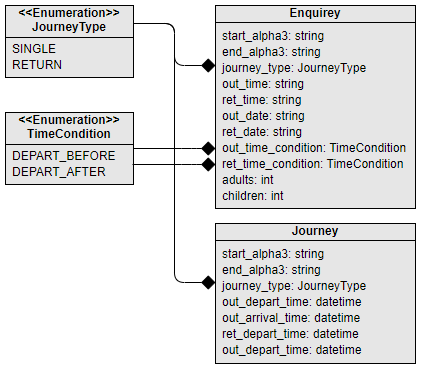
\includegraphics[width=0.5\textwidth]{images/UML_utils.png}
    \caption{Custom Types UML (\cite{visual-paradigm})}
    \label{fig:custom-types-uml}
\end{figure}


\subsection{Natural Language Processing (NLP)} \label{nlp-design}

\subsubsection{Custom Named Entity Ruler (NER)} \label{named-entity-ruler-design}

In addition to SpaCy's (\cite{spacy}) pre trained pipeline, we've injected our custom NER, into SpaCy's CNN/CPU pipeline, before it's default one, so our custom component can derive the tokens it needs, without interference. Our custom NER primarily involves a pattern set, to match station alpha3 codes to their names in natural language.

Using SpaCy's 


\subsubsection{Dialogue Flow Engine} \label{dialogue-flow-design}

We've implemented a state machine, to control the flow of conversation, dependant on it's current state compared to the data derived from tokenisation.


\subsection{Webscraping} \label{webscraping-design}


\subsection{Delay Prediction} \label{delay-prediction-design}


\subsection{User Interface} \label{user-interface-design}



% \subsubsectino()
 
% \subsection{The Architecture of the chatbot} \label{architecture}
% % You may draw a functional diagram if you like.  
% 
% % You can describe your design for each key module or component of your chatbot, in a subsection. E.g. 
% \subsection{User Interface} \label{user-interface}
% 
% \subsection{Webscraping} \label{webscraping}
% 
% % conversion of input natural language, to processable tokens
% \subsection{Natural Language Processing (NLP)} \label{nlp}
% 
% % manipulation of historical tokenized data
% \subsection{Knowledgebase} \label{knowledgebase}
% 
% % dialogue manager, state machine
% \subsection{Inferring Engine} \label{inference-engine}
% 
% % knn, K nearest neighbour, regressor, aligns to best fit
% \subsection{Delay Prediction Models} \label{delay-prediction}
% 
% \subsection{Conversation Control} \label{conversation-control}

%\begin{table}
%\centering
%\caption{This table lists ......}
%
%\begin{tabular}{|c|c|c|c|c|c|}
%\hline Methods &  &  &  &  &  \\ 
%\hline  &  &  &  &  &  \\ 
%\hline  &  &  &  &  &  \\ 
%\hline 
%\end{tabular} 
%\label{TableCC}
%\end{table}

\section{Implementation} \label{implementation}

\section{Testing} \label{testing}

\subsection{Unit Testing} \label{unit-testing}

\subsection{Integration Testing} \label{integration-testing}

\subsection{System Testing} \label{system-testing}

\subsection{Usability Testing} \label{usability-testing}


\section{Evaluation and Discussion} \label{evaluation-discussion}

\section{Conclusion} \label{conclusion}

\bibliographystyle{agsm}
%\bibliographystyle{apalike}
% you should use your own bibtex file to replace the following example_ref bib file.
\bibliography{refs} 

\end{document}
